% Figure 2 of the week-06 Oscars handout: Chrome DevTools after Inspect on
% MICHAEL B. JORDAN (oscars_devtools.png) with numbered markers on the seven
% class names the code uses. Build with `make figures` in handouts/, which
% writes oscars_devtools_annotated.pdf (PDF handout) and .png (notebook).
% Coordinates are pixels of oscars_devtools.png.
\documentclass[border=0pt]{standalone}
\makeatletter\def\input@path{{../../common/}{handouts/common/}}\makeatother
\usepackage[scaled=0.92]{helvet}
\usepackage{graphicx}
\usepackage{handoutmarkers}
\begin{document}
\setlength{\unitlength}{0.004846in}% 1 px; the figure is 5.04in wide in the handout
\begin{tikzpicture}[x=\unitlength,y=-\unitlength]
  \node[anchor=north west,inner sep=0] at (0,0)
    {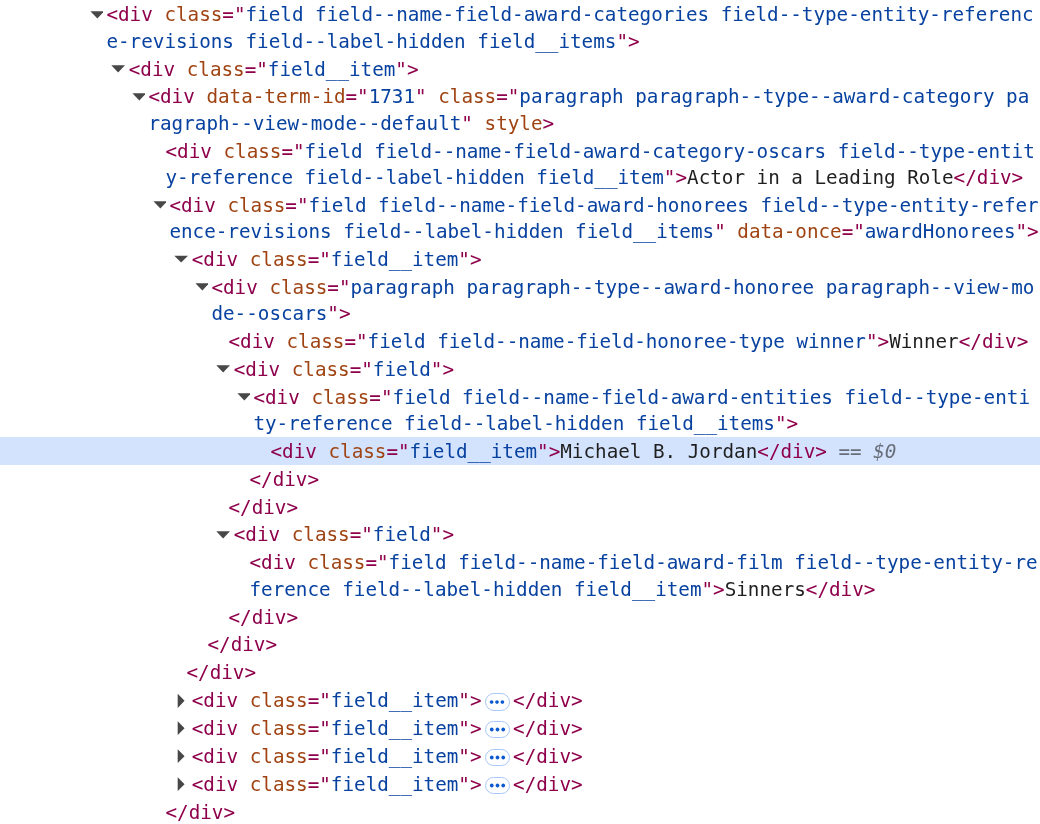
\includegraphics[width=1040\unitlength]{oscars_devtools.png}};
  \draw[black!25] (0,0) rectangle (1040,824);
  \foreach \n/\y/\x in {1/14/90, 2/96/132, 3/151/160, 4/287/195,
                        5/341/222, 6/397/237, 7/562/243} {
    \draw[marker lead] (46,\y) -- (\x,\y);
    \node[marker] at (30,\y) {\n};
  }
  % what you right-clicked
  \node[fill=white,rounded corners=2pt,inner sep=2pt,text=tab-blue,
        font=\sffamily\bfseries\scriptsize,anchor=east] at (1036,451)
        {$\leftarrow$ you clicked};
  % the four collapsed honorees
  \draw[marker brace] (596,688) -- (596,797);
  \node[anchor=west,text=tab-blue,font=\sffamily\bfseries\scriptsize]
    at (612,742) {4 more honorees \tikz[baseline=-0.6ex]\node[marker]{4};};
\end{tikzpicture}
\end{document}
